%-------------------------------%
% Biblography
%------------------------------%
\RequirePackage{filecontents}        % loading package filecontents

\def\year{2015}
%File: formatting-instruction.tex
\documentclass[letterpaper]{article}
\usepackage{aaai}
\usepackage{times}
\usepackage{helvet}
\usepackage{courier}
\frenchspacing
\setlength{\pdfpagewidth}{8.5in}
\setlength{\pdfpageheight}{11in}

\pdfinfo{
/Title (Linear-time Gibbs Sampling in Piecewise Graphical Models)
/Author (Hadi Mohasel Afshar, Scott Sanner and Ehsan Abbasnejad)}
\setcounter{secnumdepth}{0}  

\usepackage{url}
\usepackage{amsthm} %for theorems, examples, etc.
\usepackage{amsfonts} %for matbb font
\usepackage{graphicx}
\usepackage{caption} %for graphics
\usepackage{subcaption} %for graphics
\usepackage{amsmath} %for cases

\usepackage{algorithmic} %for algorithms
% Import an algorithm formatting package
\usepackage[vlined,algoruled,titlenumbered,noend]{algorithm2e}

\usepackage{verbatim} %for commenting

\newcommand{\denselist}{\itemsep 0pt\partopsep 0pt}

%\newenvironment{proof}{{\noindent\bf Proof.}}\qed%{\hspace*{\fill}\ensuremath{\diamondsuit\quad}%{\vskip 1ex}
\newtheorem{theorem}{Theorem}
\newtheorem{proposition}{Proposition}
\newtheorem{example}{Example}
\def\fexample#1#2#3{\vspace{0ex}\begin{example}[#2]\label{#1}\rm #3
\hspace*{\fill} $\diamondsuit$ \end{example}\vspace{0ex} }
\newcommand{\tuple}[1] {\langle #1 \rangle}
\newcommand{\bvec}[1]{\textbf{#1}}
\newcommand{\indicator}{\mathbb{I}}

\def\eqvsp{}  \newdimen\paravsp  \paravsp=1.3ex
\def\paradot#1{\vspace{\paravsp plus 0.5\paravsp minus 0.5\paravsp}\noindent{\bf\boldmath{#1.}}}

%\def\lgap{3.2mm}
%\newcommand{\svdots}{\vspace{-\lgap}.\vspace{-\lgap}\\.\vspace{-\lgap}\\.} 

\title{
Linear-time Gibbs Sampling in Piecewise Graphical Models
}

\author{
Hadi Mohasel Afshar\\
ANU \& NICTA\\
Canberra, Australia\\
{\tt hadi.afshar@anu.edu.au}
\And
Scott Sanner\\
NICTA \& ANU\\
Canberra, Australia\\
{\tt ssanner@nicta.com.au}
\And
Ehsan Abbasnejad\\
ANU \& NICTA\\
Canberra, Australia\\
{\tt ehsan.abbasnejad@anu.edu.au}
}

\newcommand{\fix}{\marginpar{FIX}}
\newcommand{\new}{\marginpar{NEW}}

\begin{document}

\maketitle

\begin{abstract}
Many real-world Bayesian inference problems such as preference
learning or trader valuation modeling in financial markets naturally
use piecewise likelihoods.  Unfortunately, exact closed-form inference
in the underlying Bayesian graphical models is intractable in the
general case and existing approximation techniques provide few
guarantees on both approximation quality and efficiency.  While
(Markov Chain) Monte Carlo methods provide an attractive
asymptotically unbiased approximation approach, rejection sampling and
Metropolis-Hastings both prove inefficient in practice, and analytical
derivation of Gibbs samplers require exponential space and time in the
amount of data.  In this work, we show how to transform problematic
piecewise likelihoods into equivalent mixture models and then provide
a blocked Gibbs sampling approach for this transformed model that
achieves an \emph{exponential-to-linear} reduction in space and time compared
to a conventional Gibbs sampler.  This enables fast, asymptotically
unbiased Bayesian inference in a new expressive class of piecewise graphical
models and empirically requires orders of magnitude less time than
rejection, Metropolis-Hastings, and conventional Gibbs sampling
methods to achieve the same level of accuracy.
\end{abstract}

%------------------%
%       intro         %
%------------------%
\section{Introduction}

Many Bayesian inference problems such as preference
learning~\cite{sanner:aistats10} or trader valuation modeling in
financial markets~\cite{Shogren:00} naturally use piecewise
likelihoods, e.g., preferences may induce
constraints on possible utility functions while trader transactions
constrain possible instrument valuations.  To be concrete, consider
the following Bayesian approach to preference learning where our
objective is to learn a user's weighting of attributes for
classes of items (e.g., cars, apartment rentals, movies) given their
responses to pairwise comparison queries over those items:

%%%%%%%%%%%%%%%%%%%%%%%%%
\begin{figure*}%[t!]
\begin{subfigure}{.19\textwidth}
\centering
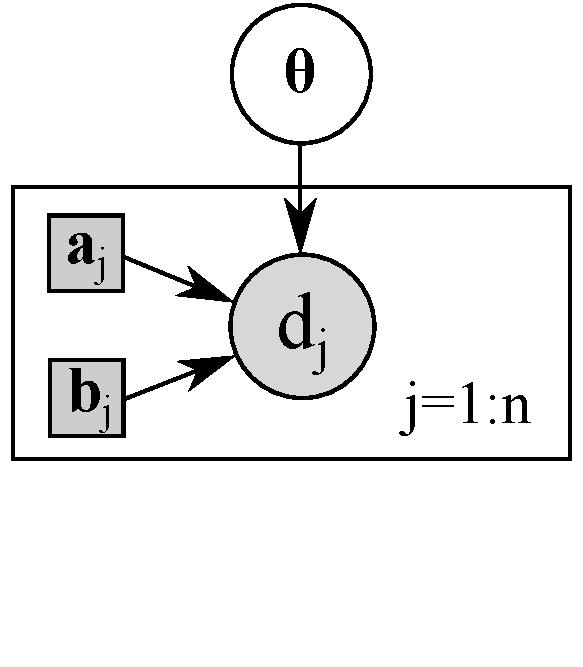
\includegraphics[width=1.0\textwidth]{pic/pref2ww.pdf}
\vspace{-6mm}
\caption{}
\end{subfigure}
\begin{subfigure}{.795\textwidth}
\centering
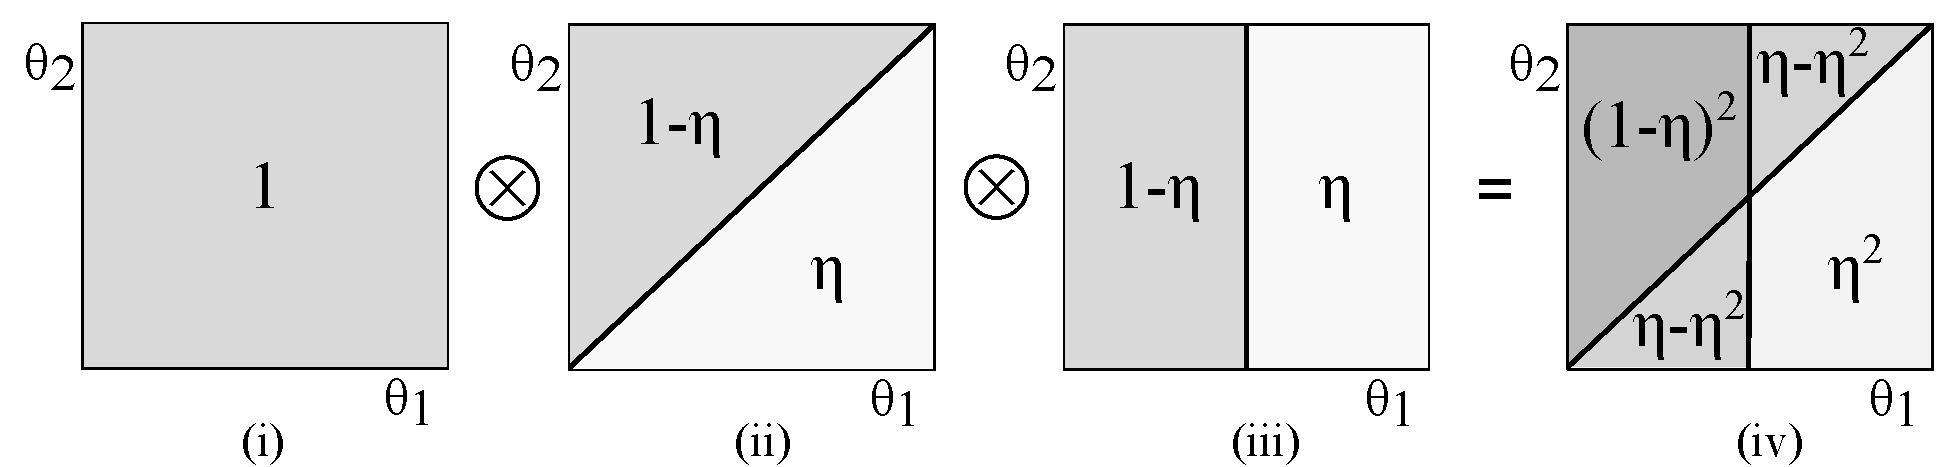
\includegraphics[width=1.0\textwidth]{pic/running1.pdf}
\label{fig:pref}
\vspace{-1mm}
\caption{}
\end{subfigure}
\vspace{-2mm}
\caption{\footnotesize 
(a) Graphical model for BPPL problem in Example \ref{example:pref}.
(b) A 2D instance of Example \ref{example:pref}: 
(i) An (unnormalized) prior uniform in a rectangle with center (0,0).
(ii) Likelihood model $pr(\bvec{a}_1 \succ \bvec{b}_1 | \, \boldsymbol\theta)$ and
(iii) $pr(\bvec{a}_2 \succ \bvec{b}_2 | \, \boldsymbol\theta)$ 
(as in Eq.~\ref{e:pref1likelihood}) where
$\bvec{a}_1 = (5, 3)$, $\bvec{b}_1 = (6, 2)$, $\bvec{a}_2 = \bvec{a}_1$ and $\bvec{b}_2 = (6, 3)$.
(iv) A piecewise function proportional to the posterior distribution.}
\label{fig:pref-up-down}
\end{figure*}
%%%%%%%%%%%%%%%%%%%%%%%%%
\fexample{example:pref}{Bayesian pairwise preference learning (BPPL)}{
  Suppose each \emph{item} $\bvec{a}$ is modeled by an $D$-dimensional
  real-valued \emph{attribute choice vector} $(\alpha_1, \ldots,
  \alpha_D)$.  The goal is to learn an \emph{attribute weight vector}
  $\boldsymbol\theta = (\theta_1, \ldots, \theta_D) \in \mathbb{R}^D$
  that describes the utility of each attribute choice from user
  responses to preference queries.  As commonly done in
  \emph{multi-attribute utility theory} \cite{Keeney:93}, the overall
  item utility $u(\bvec{a}|\, \boldsymbol\theta)$ is decomposed 
  additively over the attribute choices of $\bvec{a}$:
%
$$
u(\bvec{a} | \, \boldsymbol\theta) = \sum_{i=1}^D \theta_i\cdot\alpha_i
$$
%
User responses are in the form of $n$ queries (i.e.\ observed data
points) $d_1$ to $d_n$ where for each $1\leq j \leq n$, $d_j$ is a pairwise comparison of some
items $\bvec{a}_j$ and $\bvec{b}_j$ with the following possible
responses:
\begin{itemize}\denselist
\item {\small $\bvec{a}_j \succ \bvec{b}_j$}:  In the $j$-th query, the user prefers item {\small$\bvec{a}_j$} over {\small$\bvec{b}_j$}.
\item {\small $\bvec{a}_j \preceq \bvec{b}_j$}:  In the $j$-th query, the user does not prefer item {\small $\bvec{a}_j$} over {\small$\bvec{b}_j$}.
\end{itemize}
It is assumed that with an \emph{elicitation noise} $0 \leq \eta <
0.5$, the item with a greater utility is preferred:
\begin{align}
\label{e:pref1likelihood}
pr(\bvec{a}_j \succ \bvec{b}_j \,|\, \boldsymbol\theta) =
{\footnotesize
\begin{cases}
u(\bvec{a}_j|\boldsymbol\theta) < u(\bvec{b}_j|\boldsymbol\theta) : \eta\\
u(\bvec{a}_j|\boldsymbol\theta) = u(\bvec{b}_j|\boldsymbol\theta) : 0.5\\
u(\bvec{a}_j|\boldsymbol\theta) > u(\bvec{b}_j|\boldsymbol\theta) : 1-\eta
\end{cases}
}%end footnote size
\\
pr(\bvec{a}_j \preceq \bvec{b}_j \,|\, \boldsymbol\theta) = 
1 - pr(\bvec{a}_j \succ \bvec{b}_j \,|\, \boldsymbol\theta)
\end{align}
As the graphical model in Figure~\ref{fig:pref-up-down} illustrates, our posterior
belief over the user's attribute weights is provided by the standard
Bayesian inference expression:
$
pr(\boldsymbol\theta | \, d_1, \ldots, d_n) 
\propto pr(\boldsymbol\theta) \cdot \prod_{j=1}^{n} pr(d_j | \, \boldsymbol\theta)
$. As also evidenced in Figure~\ref{fig:pref-up-down}, since the
prior and likelihoods are piecewise distribitions, the posterior
distribution is also piecewise with the number of pieces growing exponentially
in $n$.  
} %end example 1
%\vspace{2mm}
%%%%%%%%%%%%%%%%%%%%%%%%%%%%%%%%%%%%%%%%

Unfortunately, Bayesian inference in models with piecewise likelihoods
like BPPL in Example~\ref{example:pref} (and illustrated in
Figure~\ref{fig:pref-up-down}) often lead to posterior distributions
with a number of piecewise partitions \emph{exponential in the number
  of data points}, thus rendering exact analytical
inference impossible.  While (Markov Chain) Monte Carlo methods
\cite{gilks2005markov}
provide an attractive asymptotically unbiased approximation approach,
rejection sampling and Metropolis-Hastings \cite{hastings1970monte} both prove inefficient in
practice, and analytical derivation of Gibbs samplers \cite{casella1992explaining} require
exponential space and time in the number of data points.

In this work, we show how to transform problematic
piecewise likelihoods into equivalent mixture models and provide
a blocked Gibbs sampling approach for this transformed model that
achieves an \emph{exponential-to-linear} reduction in space and time compared
to a conventional Gibbs sampler.  This enables fast, asymptotically
unbiased Bayesian inference in a new expressive class of piecewise graphical
models and empirically requires orders of magnitude less time than
rejection, Metropolis-Hastings, and conventional Gibbs sampling
methods to achieve the same level of accuracy -- especially
when the number of posterior partitions grows rapidly in the number of observed data points.

After a brief introduction to piecewise models and the
exact/asymptotically unbiased inference methods that can be applied to 
them in the following section, a novel inference 
algorithm (referred to as \emph{Augmented Gibbs} sampling throughout)
is presented.



%--------------------------------%
%      Bayesian inference      %
%--------------------------------%

\section{Bayesian Inference on Graphical Models with Piecewise Distributions}
\label{sec:inference_piecewise_models}
\subsubsection{Inference.} 
We will present an inference method that can be generalized to  
a variety of graphical models with piecewise factors, however, our focus in this
work is on Bayesian networks factorized in the following
standard form: 
{\footnotesize
\begin{equation}
\label{e:posterior}
pr(\boldsymbol\theta | \, d_1, \ldots, d_n) 
\propto
pr(\boldsymbol\theta, \, d_1, \ldots, d_n) 
= pr(\boldsymbol\theta) \cdot \prod_{j=1}^{n} pr(d_j | \boldsymbol\theta) 
\end{equation}
} 
\!\!where $\boldsymbol\theta := (\theta_1, \ldots, \theta_D)$ is a parameter vector and $d_j$ are observed data points. 
A typical inference task 
with this posterior distribution is to compute the expectation of a function of $f(\boldsymbol\theta)$ given data:
\begin{equation}
\label{e:prob.outcome}
\mathbb{E}_{\boldsymbol\theta}[f(\boldsymbol\theta) \,|\, d_1, \ldots, d_n \,]
\end{equation}


\subsubsection{Piecewise Models.}%\paradot{Piecewise Models} 
We are interested in the inference on models where prior/likelihoods are piecewise.
A function {\small$f(\boldsymbol{\theta})$} is {\small$N$}\!-piece \emph{piecewise} if it can be represented as:
\begin{equation}
\label{e:piecewise}
f(\boldsymbol{\theta}) = 
{\footnotesize
\begin{cases}
\phi_1(\boldsymbol{\theta}) : & f_1(\boldsymbol{\theta})\\
\vdots\\
\phi_N(\boldsymbol{\theta}) : & f_N(\boldsymbol{\theta})
\end{cases}
}%end footnote size
\end{equation}
where $\phi_1$ to $\phi_N$ are mutually exclusive and jointly exhaustive Boolean functions (constraints) 
that partition the space of variables $\boldsymbol{\theta}$. If for a particular variable assignment $\boldsymbol{\theta}^{(0)}$ and $1\leq v \leq N$, constraint 
$\phi_v(\boldsymbol{\theta}^{(0)})$ is satisfied, then by definition, the function returns the value of its $v$-th \emph{sub-function}: $f(\boldsymbol{\theta}^{(0)}) = f_v(\boldsymbol{\theta}^{(0)})$.  
In this case, it is said that sub-function $f_v$ is \emph{activated} by assignment $\boldsymbol{\theta}^{(0)}$.


In the implementation of our proposed algorithm, the constraints are restricted to linear/quadratic (in)equalities while sub-functions are polynomials with real exponents. 
However, in theory, the algorithm can be applied to \emph{any} family of piecewise models in which the roots of univariate constraint expressions can be found and sub-functions (and their products) are integrable. 

\subsubsection{Complexity of Inference on Piecewise Models.}
If in the model of Equation \ref{e:posterior}, the prior $pr(\boldsymbol\theta)$ 
is an $L$-piece distribution and each of the $n$ likelihoods is a piecewise function with number of partitions  bound by $M$, 
then the joint distribution is a piecewise function with number of partitions bound by $LM^n$ (therefore, $O(M^n)$).
The reason, as clarified by the following simple formula,   
is that the number of partitions in the product of two piecewise functions is bound by the product of their number of partitions:\footnote{
If pruning potential inconsistent (infeasible) constraint is possible
(i.e.\ by \emph{linear constraint solvers} for linear constrains) and the imposed extra costs are justified,
the number of partitions may be less.
}%endfootnote

{\footnotesize
\begin{align*}
&\begin{cases}
\!\phi_1(\boldsymbol{\theta}) \!: &\!\!\!\!\! f_1(\boldsymbol{\theta})\\
\!\phi_2(\boldsymbol{\theta}) \!: &\!\!\!\!\! f_2(\boldsymbol{\theta})
\end{cases}
\!\otimes\!
\begin{cases}
\!\psi_1(\boldsymbol{\theta}) \!: &\!\!\!\!\! g_1(\boldsymbol{\theta})\\
\!\psi_2(\boldsymbol{\theta}) \!: &\!\!\!\!\! g_2(\boldsymbol{\theta})
\end{cases}
\!\!=\!
\begin{cases}
\!\phi_1(\boldsymbol{\theta}) \wedge \psi_1(\boldsymbol{\theta}) \! :\!\!\!\!\! & f_1(\boldsymbol{\theta}) g_1(\boldsymbol{\theta})\\
\!\phi_1(\boldsymbol{\theta}) \wedge \psi_2(\boldsymbol{\theta}) \! :\!\!\!\!\! & f_1(\boldsymbol{\theta}) g_2(\boldsymbol{\theta})\\
\!\phi_2(\boldsymbol{\theta}) \wedge \psi_1(\boldsymbol{\theta}) \! :\!\!\!\!\! & f_2(\boldsymbol{\theta}) g_1(\boldsymbol{\theta})\\
\!\phi_2(\boldsymbol{\theta}) \wedge \psi_2(\boldsymbol{\theta}) \! :\!\!\!\!\! & f_2(\boldsymbol{\theta}) g_2(\boldsymbol{\theta})
\end{cases}
\end{align*}
}%end footnote size
\subsubsection{Exact Inference on Piecewise Models.} In theory, closed-form inference on piecewise models (at least piecewise polynomials) with linear constraints is possible \cite{Sanner:12}.
In practice, however, such symbolic methods rapidly become intractable since the posterior requires
the representation of $O(M^n)$ distinct case partitions.
 
\subsubsection{Approximate Inference on Piecewise Modes.} 
An alternative option is to seek \emph{asymptotically unbiased} inference methods
via Monte Carlo sampling.
Given a set of $S$ samples (particles) $\{\boldsymbol\theta^{(1)}, \ldots, \boldsymbol\theta^{(S)}\}$ taken from a posterior $pr(\boldsymbol\theta | \, d_1, \ldots, d_n)$, 
the inference task of Equation~\ref{e:prob.outcome} can be approximated by: 
$\frac{1}{S} \sum_{s=1}^S f(\boldsymbol\theta^{(s)} | \, d_1, \ldots, d_n)$.
Three widely used sampling methods for an arbitrary distribution $pr(\boldsymbol\theta | \, d_1, \ldots, d_n)$ are the following:

\emph{Rejection sampling}:
Let $p(\boldsymbol{\theta})$ and $q(\boldsymbol{\theta})$ be two distributions 
such that direct sampling from them is respectively hard and easy
and
$p(\boldsymbol{\theta})/q(\boldsymbol{\theta})$ is bound by a constant $c>1$. 
To take a sample from $p$ using \emph{rejection sampling}, 
a sample $\boldsymbol{\theta}$ is taken from distribution $q$ and accepted with probability $p(\boldsymbol{\theta}) / c q(\boldsymbol{\theta})$, 
otherwise it is rejected and the process is repeated. 
If $c$ is too large, the speed of this algorithm is slow since often lots of samples are required until one is accepted.

\emph{Metropolis-Hastings (MH)}:
To generate a Markov Chain Monte Carlo (MCMC) 
sample $\boldsymbol{\theta}^{(t)}$ from a distribution $p(\boldsymbol{\theta})$ given a previously taken sample $\boldsymbol{\theta}^{(t-1)}$, 
firstly, a sample $\boldsymbol{\theta}'$ is taken 
from a symmetric \emph{proposal density} $q(\boldsymbol{\theta} |\, \boldsymbol{\theta}^{(t-1)})$ 
%from which samples can be taken efficiently 
(often an isotropic \emph{Gaussian} centered at $\boldsymbol{\theta}^{(t-1)}$). 
With probability 
{\footnotesize
$\min \big(1, q(\boldsymbol{\theta}^{(t-1)}|\boldsymbol{\theta}')p(\boldsymbol{\theta}')/q(\boldsymbol{\theta}'|\boldsymbol{\theta}^{(t-1)})p(\boldsymbol{\theta}^{(t-1)}) \big)$
}, 
$\boldsymbol{\theta}'$ is accepted $\boldsymbol{\theta}^{(t)} \leftarrow \boldsymbol{\theta}'$, otherwise, $\boldsymbol{\theta}^{(t)} \leftarrow \boldsymbol{\theta}^{(t-1)}$. 
Choosing a good \emph{proposal} is problem-dependent and requires tuning. Also most of proposals that often require costly posterior evaluation is rejected leading to a poor performance. 


\emph{Gibbs sampling}:
A celebrated MCMC method in which generating new samples $\boldsymbol{\theta} = ({\theta}_1, \ldots, {\theta}_D)$ requires each variable $\theta_i$ to be sampled conditioned on
the last instantiated value of the others:\footnote{
This paper deals with piecewise polynomial distributions. For such distributions, the CDF of $p(\theta_i | \, \boldsymbol\theta_{-i})$
(which is a univariate piecewise polynomial)
 is computed analytically. 
To approximate CDF$^{-1}$ which is required for sampling $\theta_i$ (via \emph{inverse transform sampling}), in each step of Gibbs sampling \emph{binary search} is used.
} %end footnote.
\begin{equation}
\label{eq:gibbs}
{\theta}_i \sim p({\theta}_i | \, \boldsymbol{\theta}_{-i})
\end{equation} 

Computation of $D$ univariate \emph{cumulative distribution functions} (CDFs) 
(one for each $p({\theta}_i | \, \boldsymbol{\theta}_{-i})$) as well as their inverse functions is required which can be quite time consuming. 
In practice, when these integrals are not tractable or easy to compute Gibbs sampling can be prohibitively expensive.   

Compared to rejection sampling or MH, the performance of Gibbs sampling on the aforementioned \emph{piecewise} models is exponential in the number of observations.  
In this work, we propose an alternative linear Gibbs sampler.


%---------------------------%
%          Mixture              %
%---------------------------%
\section{Piecewise Models as Mixture Models}
\label{sect:mix}

%%%%%%%%%%%%%%%%%%%%%%%%%
\begin{figure}
\centering
\begin{subfigure}{.45\linewidth} %48
\centering
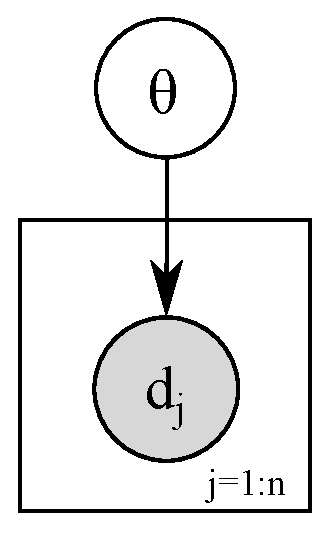
\includegraphics[width=.56\textwidth]{pic/naive.pdf}
\caption{}
\label{fig:naive}
\end{subfigure}
\begin{subfigure}{.45\linewidth}
\centering
  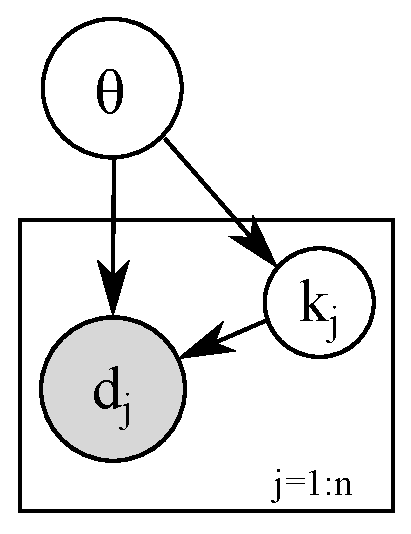
\includegraphics[width=.70\textwidth]{pic/naive-mix2.pdf}
\caption{}
\label{fig:naive.mix}
\end{subfigure}
\vspace{-3mm}
\caption{\footnotesize 
(a) A Bayesian inference model with parameter (vector) $\boldsymbol\theta$ and data points $d_1$ to $d_n$.
(b) A mixture model with parameter (vector) $\boldsymbol\theta$ and data points $d_1$ to $d_n$ 
}
\vspace{-5mm}
\end{figure}
%%%%%%%%%%%%%%%%%%%%%%%

In this section we detail how to overcome the exponential complexity of standard Gibbs
sampling by transforming piecewise models to (augmented) mixture models and performing
linear time Gibbs sampling in the latter models. 
While augmented models to facilitate
Gibbs sampling have been proposed previously, e.g., Swendsen-Wang (SW) sampling~\cite{sw_mc} 
and more recently FlyMC sampling~\cite{fly_mc}, methods like SW are specific to restricted
Ising models and FlyMC requires careful problem-specific proposal design and tuning.  In this paper,
we present a generic augmented model for an expressive class of piecewise models and
an analytical Gibbs sampler that does not require problem-specific proposal design.  
Furthermore, our Augmented Gibbs proposal achieves a novel \emph{exponential-to-linear reduction} in the complexity
of sampling from a Bayesian posterior with an exponential number of pieces.

We motivate the algorithm by first introducing the augmented posterior for piecewise likelihoods:
{\small
\begin{align*}
&pr(\boldsymbol\theta | \, d_1, \ldots, d_n) \, 
\propto 
pr(\boldsymbol\theta) \; \otimes
\\
&%{\footnotesize
\begin{cases}
\boxed{k_1 = 1.} \;\;\, {\phi^{1}_{1}(\boldsymbol\theta)  : f^{1}_{1}(\boldsymbol\theta)}\\
\vdots
\\
\boxed{k_1 = M.} \, \phi^{1}_{M}(\boldsymbol\theta)  \!:\! f^{1}_{M}(\boldsymbol\theta)
\end{cases}
%}%end font size
\!\!\!\!\!\!\!\!\!\!\!\!\!
\otimes
\cdots
\otimes
%{\footnotesize
\begin{cases}
\boxed{k_n = 1.} \;\;\, \phi^{n}_{1}(\boldsymbol\theta)  : f^{n}_{1}(\boldsymbol\theta)\\
\vdots
\\
\boxed{k_n = M.} \, \phi^{n}_{M}(\boldsymbol\theta)  \!:\! f^{n}_{M}(\boldsymbol\theta)
\end{cases}
%}%end font size
\end{align*} 
}%end small
%\footnote{Clearly, prior distributions can be piecewise as well but since exponential blow up in the posterior structure is due to the amount of data, our focus is on likelihood functions.}
In the above, $k_j$ is the partition-counter of the $j$-th likelihood function. 
$\phi^j_{v}$ is its $v$-th constraint and
 $f^j_{v}$ is its associated sub-function. 
 Also for readability, case statements are numbered and without loss of
generality, we assume the number of partitions in each
likelihood function is $M$.

We observe that each $k_j$ can be seen as a random variable. 
It deterministically takes the value of the partition whose associated constraint holds (given $\boldsymbol\theta$) and its possible outcomes are in $\textsc{Val}(k_j) = \{1, \ldots, M\}$. 
Note that for any given $\boldsymbol\theta$, exactly one constraint holds for a piecewise function, therefore, 
$\sum_{k_j = 1}^M pr(k_j \,|\, \boldsymbol\theta) = 1$.
Intuitively, it can be assumed that $k_j$ is the underlying variable that determines which partition of each likelihood function is `chosen'. As we have: 
{\small
\begin{equation}
\label{e:aaaax}
pr(d_j | \, \boldsymbol\theta) = \sum_{k_j = 1}^M pr(k_j | \, \boldsymbol\theta) pr(d_j | \, k_j, \boldsymbol\theta) 
\end{equation}
}%small
we can claim that a piecewise likelihood function is a mixture model in which sub-functions $f^j_v$ are the \emph{mixture components} and 
 $k_j$ provide binary \emph{mixture weights}. Hence:
{\small
\begin{align*}
pr(\boldsymbol\theta | \, d_1, \ldots, d_n) 
&\propto
pr(\boldsymbol\theta) \otimes
\sum_{k_1}pr(k_1 | \, \boldsymbol\theta) pr(d_1 | \, k_1, \boldsymbol\theta) \\
&\qquad\qquad \otimes
\cdots \otimes
\sum_{k_n}pr(k_n | \, \boldsymbol\theta) pr(d_n | \, k_n, \boldsymbol\theta)
\\
&\propto
\sum_{k_1} \ldots \sum_{k_n} p(\boldsymbol\theta, d_1, \ldots, d_n, k_1, \ldots, k_n) 
\end{align*}}
This means that the Bayesian networks in Figures~\ref{fig:naive} and \ref{fig:naive.mix} are equivalent.
Therefore, instead of taking samples from \ref{fig:naive}, 
they can be taken from the \emph{augmented model} \ref{fig:naive.mix}. A key observation, however, is that 
unlike the conditional distributions $pr(\theta_i | \, \boldsymbol\theta_{-i})$, 
in $pr(\theta_i | \boldsymbol\theta_{-i}, k_1, \ldots, k_n)$ 
the number of partitions is constant rather than growing as $M^n$.

The reason is that if  $\bvec{k}= (k_1, \ldots, k_n)$ are given, for the $j$-th 
likelihood a single sub-function $f^j_{k_j}$ is `chosen' and
$pr(\theta_i | \, \boldsymbol\theta_{-i}, k_1, \ldots, k_n) \propto
pr(\theta_i | \, \boldsymbol\theta_{-i})
\prod_{j=1}^n f^j_{k_j}(\boldsymbol\theta)$.
Since the sub-functions are not piecewise themselves, 
the number of partitions in $pr(\theta_i |\, \boldsymbol\theta_{-i},  k_1, \ldots, k_n)$ is bound by the number of partitions in the prior.

In the following proposition, we prove Equation~\ref{e:aaaax} is valid:
%
\begin{proposition}
\label{pro:discrete}
The following likelihood function:
{\footnotesize
\begin{equation}
pr(d | \, \boldsymbol\theta) := 
\begin{cases}
\phi_1(\boldsymbol\theta)  &\!\!\!\!: f_1(\boldsymbol\theta)\\
									  &\!\!\!\!\vdots\\
\phi_M(\boldsymbol\theta)  &\!\!\!\!: f_M(\boldsymbol\theta)
\end{cases}
\label{e:piecewise.likelihood22}
\end{equation}
}
is equivalent to 
$\sum_{k = 1}^M pr(k | \, \boldsymbol\theta) pr(d | \, k, \boldsymbol\theta)$
where:
{\footnotesize
\begin{equation}
\label{e:2rel2299}
pr(k |\, \boldsymbol\theta) := 
\begin{cases}
\phi_k(\boldsymbol\theta)  &\!\!\!\!: 1\\
\neg \phi_k(\boldsymbol\theta) &\!\!\!\!: 0
\end{cases}
\qquad \quad
pr(d | \, k, \boldsymbol\theta) := f_k(\boldsymbol\theta)
\end{equation}
}
\end{proposition}


\begin{proof}
Since constraints $\phi_k$ are mutually exclusive and jointly exhaustive: 
{\footnotesize
$$\sum_{k= 1}^M pr(k | \, \boldsymbol\theta) = 
\sum_{k=1}^M
\begin{cases}
\phi_k(\boldsymbol\theta)   &: 1\\
\neg \phi_k(\boldsymbol\theta)  &: 0
\end{cases}
\, =1
$$
}
Therefore $pr(k | \, \boldsymbol\theta)$ is a proper probability function. 
On the other hand, by marginalizing $k$, (\ref{e:2rel2299})
trivially lead to (\ref{e:piecewise.likelihood22}):
%
{\small 
\begin{align*}
\sum_{k} pr(k | \, \boldsymbol\theta) pr(d | \, k, \boldsymbol\theta) 
&= 
\sum_{k=1}^M  
{\footnotesize
\begin{cases}
\phi_k(\boldsymbol\theta)         &\!\!\!\!\!: 1\\
\neg \phi_k(\boldsymbol\theta) &\!\!\!\!\!: 0
\end{cases}
}%end font size
 \cdot f_k(\boldsymbol \theta)
,&&\text{by (\ref{e:2rel2299})}
\\
=
\sum_{k=1}^M
{\footnotesize
\begin{cases}
		\phi_k(\boldsymbol\theta)  &\!\!\!\!\!: \! f_k(\boldsymbol\theta)\\
\neg 	\phi_k(\boldsymbol\theta)  &\!\!\!\!\!:           \! 0
\end{cases}
}%end font size
%\nonumber \\
\!&= {\footnotesize
\begin{cases}
\phi_1(\boldsymbol\theta)  &\!\!\!\!\!:\! f_1(\boldsymbol\theta)\\
\vdots\\
\phi_M(\boldsymbol\theta)  &\!\!\!\!\!:\! f_M(\boldsymbol\theta)
\end{cases}
}%end font size
\!\!= pr(d | \, \boldsymbol\theta) 
&&\text{by (\ref{e:piecewise.likelihood22})}
\end{align*}}
in which the third equality holds since constraints $\phi_k$ are mutually exclusive. 
\end{proof}
 
\subsection{Deterministic Dependencies and Blocked Sampling}
\label{sect:deterministic}
%%%%%%%%%%%%%%%%%%%%%%%%%
\begin{figure}
  \centering
  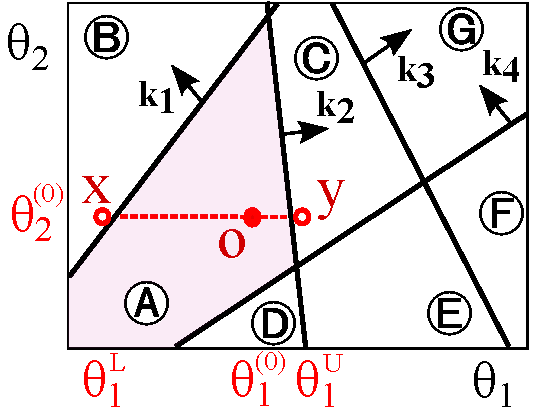
\includegraphics[width=0.22\textwidth]{pic/colxx.pdf}
\vspace{-1mm}
\caption{\footnotesize
A piecewise joint distribution of $(\theta_1, \theta_2)$ partitioned by bi-valued linear constraints.
In the side, specified by each arrow, its associated auxiliary variable $k_j$ is 1 otherwise 2.
A Gibbs sampler started from an initial point $O = (\theta_1^{(0)}, \theta_2^{(0)})$, is trapped in an initial partition (A) 
where $k_1 = k_2 = k_3 = 2$ and $k_4 = 1$. 
}
\label{fig:simple.example}
\end{figure}
%%%%%%%%%%%%%%%%%%%%%%%
It is known that in the presence of determinism Gibbs sampling gives poor results \cite{Poon:06}.
In our setting, deterministic dependencies arise from the definition of $pr(k |\, \boldsymbol\theta)$ in (\ref{e:2rel2299}), were the value of $k$ is  decided by $\boldsymbol{\theta}$.
This problem is illustrated in Figure~\ref{fig:simple.example} by a simple example:
A Gibbs sampler started from an initial point $O=(\theta_1^{(0)}, \theta_2^{(0)})$, 
is trapped in the initial partition (A). 
The reason is that conditioned on the initial value of the auxiliary variables, 
the partition is deterministically decided as being (A), and conditioned on any 
point in (A), the auxiliary variables keep their initial values. %I.e.\ only on 
%%%%%%%%%%%%%%%%%%%%%%%%%%%%%%%%%%%%%%%%%%%%%%%%%%%%%%%%%%%%%%%%%%%%%%%%%%%%%%%%%%%%%%%%%%%
%% NOTE TO HADI: need to define the sampler!  Symbolic CDF then binary search for inverse!
%%               also need to clean up conditioning on data; also partition for datum d?
%%%%%%%%%%%%%%%%%%%%%%%%%%%%%%%%%%%%%%%%%%%%%%%%%%%%%%%%%%%%%%%%%%%%%%%%%%%%%%%%%%%%%%%%%%%

\paradot{Blocked Gibbs}
We avoid deterministic dependencies by Blocked sampling:
at each step of Gibbs sampling, a parameter variable $\theta_i$ is 
jointly sampled with  
(at least) one auxiliary variable $k_j$ 
conditioned on the remaining variables:
{\small
$$
(\theta_i, k_j) \sim pr(\theta_i, k_j | \, \boldsymbol 
\theta_{-i}, 
\bvec{k}_{-j})  
$$
}
This is done in 2 steps:
\begin{enumerate}
% \setlength\itemsep{0em}
\item 
$k_j$ is marginalized out and $\theta_i$ is sampled (\emph{collapsed 
Gibbs sampling}):
{\footnotesize
$$
\theta_i \sim \sum_{k_j} 
pr(k_j | \, \boldsymbol \theta_{-i}, \bvec{k}_{-j}) 
pr(\theta_i | \, k_j, \boldsymbol \theta_{-i}, \bvec{k}_{-j})  
$$
}
\item
The value of $k_j$ is deterministically found given $\boldsymbol \theta$:\\
$k_j \leftarrow v \in \textsc{Val}(k_j)$ s.t.\ 
$\phi_v^j(\boldsymbol \theta) = \textit{true}$
where $\phi_v^j$ is the $v$-th constraint of the $j$-th likelihood function.
\end{enumerate}

For instance in Figure~\ref{fig:simple.example}, if for sampling $\theta_2$, 
$k_1$ (or $k_2$) is collapsed,
then the next sample will be in the union of partition (A) and (B) (resp. the union of (A) and (C)). 

\paradot{Targeted Selection of Collapsed Auxiliary Variables}
We provide a mechanism for finding auxiliary variables $k_j$ that are not determined by the other auxiliary variables, 
$\bvec{k}_{-j}$ when jointly sampled with a parameter variable 
$\theta_i$. 
We observe that the set of partitions satisfying the current valuation of $\bvec{k}$
often differs with its adjacent partitions in a single auxiliary variable.
Since such a variable is not determined by other variables, it can be used in 
the blocked sampling.

However, in case some likelihood functions share the same constraint, some 
adjacent partitions would differ in multiple auxiliary variables.
In such cases, more than one auxiliary variable should be used in blocked sampling.

Finding such auxiliary variables has a simple geometric interpretation. As 
such, we explain it by a simple 
example depicted in Figure~\ref{fig:simple.example}.
Consider finding a proper $k_j$ 
for blocked sampling $pr(\theta_1, k_j | \, 
\theta_2^{(0)}, \bvec{k}_{-j})$. 
It suffices to pass the end points of the (red dotted) line segment 
$pr(\theta_1 | \, \theta_2^{(0)}, \bvec{k})>0$ by an extremely small value $\varepsilon$ to end in points 
$x=(\theta_1^L, \theta_2^{(0)})$ and $y = (\theta_1^U, \theta_2^{(0)})$ 
in partitions (B) and (C).\footnote{More generally,  
$\theta_i^L := \inf   \{ \theta_i \,|\,\, p(\theta_i | \, \boldsymbol{\theta}_{-i}, \bvec{k})>0 \} - \varepsilon$
and $\theta_i^U := \sup \{ \theta_i \,|\,\, p(\theta_i | \, \boldsymbol{\theta}_{-i}, \bvec{k})>0 \} + \varepsilon$ where $0<\varepsilon \ll 1$.
}
In this way, the neighboring partitions and consequently 
their corresponding $\bvec{k}$ valuations are detected. 
Finally, the auxiliary variables that differ between (A) and (B) or differ between (A) and (C) are found ($k_1$ and $k_2$, in Figure~\ref{fig:simple.example}). 


%------------------------%
%      experiments      %
%------------------------%
\section{Experimental Results}
\label{sect:experiment}

In this section we show that the mixing time of the proposed method, \emph{augmented Gibbs} sampling, is faster than Rejection sampling, baseline 
Gibbs and MH.     
Algorithms are tested against the BPPL model of Example~\ref{example:pref} and a \emph{Market maker} (MM) model motivated by \cite{Das:08}:
%%%%%%%%%%%%%%%%%
\begin{figure}
\centering
\begin{subfigure}{.35\textwidth}
\centering
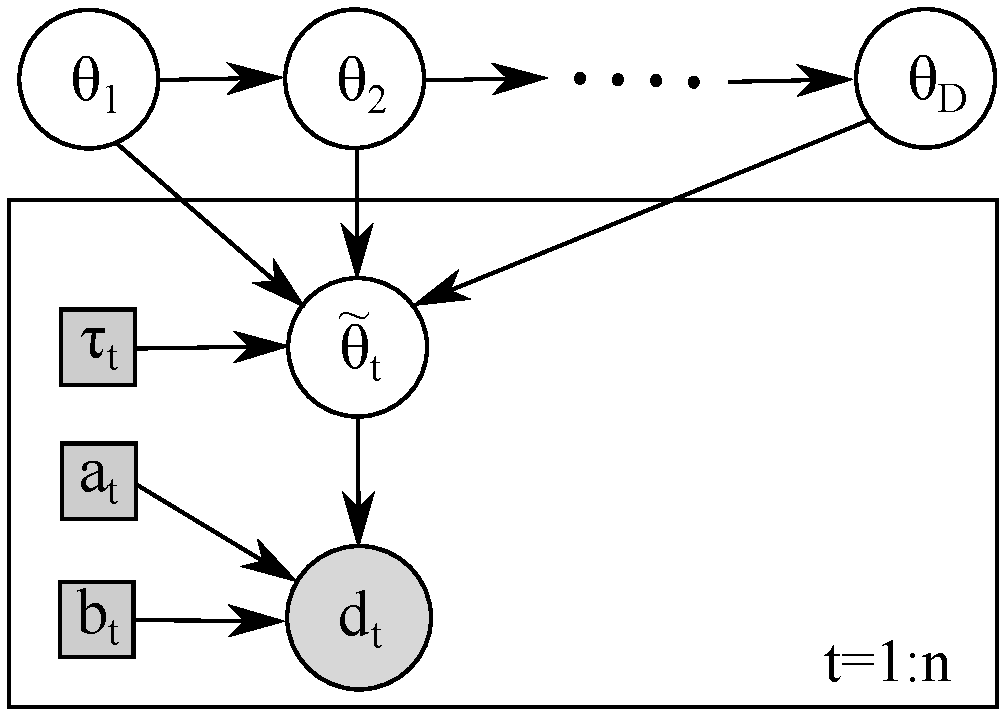
\includegraphics[width=.90\textwidth]{pic/market4w.pdf}
\caption{}
\label{fig:market}
\end{subfigure}
\begin{subfigure}{.24\textwidth}
  \centering
  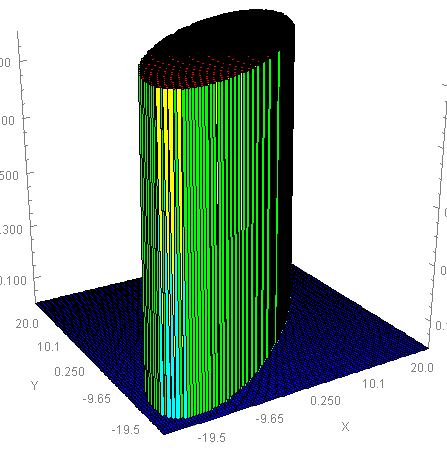
\includegraphics[width=.82\textwidth]{pic/elipsePrior.png}
  \caption{}
  \label{fig:mmm.prior}
\end{subfigure}%
\begin{subfigure}{.24\textwidth}
  \centering
  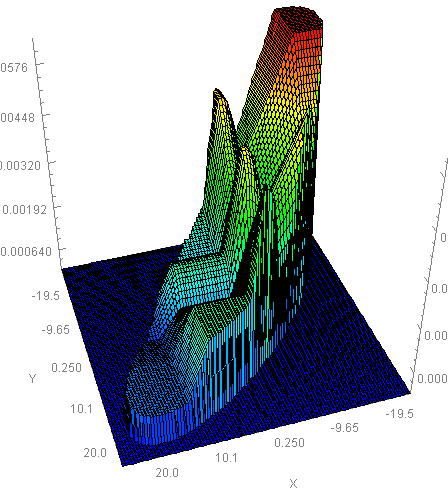
\includegraphics[width=.80\textwidth]{pic/MM2.png}
  \caption{}
  \label{fig:mmm.posterior}
\end{subfigure}
\vspace{-1mm}
\caption{\footnotesize 
Market Maker problem of Example~\ref{example:market}.
(a) Prior distribution of two instrument types (therefore, a 2D space). 
(b) Corresponding posterior given 4 observed data points (trader responses).}
\label{fig:mmm}
\end{figure}
%%%%%%%%%%%%%%%%%

%\vspace{1mm}
\fexample{example:market}{Market maker (MM)}{
Suppose there are $D$ different types of \emph{instruments} with 
respective valuations 
$\boldsymbol\theta=(\theta_{1}, \ldots,  \theta_{D})$.
There is a \emph{market maker} 
who at each time step $t$ deals an instrument of type $\tau_t \in \{1, 
\ldots, D\}$ by setting \emph{bid} and \emph{ask} $b_{t}$ and $a_{t}$ denoting 
prices at which she is willing to buy and sell each unit respectively 
(where $b_{t} \leq a_{t}$).
The ``true" valuation of different types
are unknown (to her) but any a priori knowledge over their dependencies that can be expressed via a DAG structure over their associated random variables is permitted.
Nonetheless, without loss of generality we only consider the following simple dependency:  
Assume the types indicate different versions of the same product and
each new version is more expensive than the older ones 
($\theta_{i} \leq \theta_{i+1}$).
The valuation of the oldest version is within some given price range $[L, H]$
and the price difference of any consecutive versions is bound by a known parameter $\delta$:
%
\begin{align*}
pr(\theta_{1})     &= \mathcal{U}(L, H) \qquad \qquad\\
pr(\theta_{i+1})  &= \mathcal{U}(\theta_{i}, \theta_{i} + \delta) \quad \forall i \in \{1, \ldots, D-1\}
\end{align*} 
%
where $\mathcal{U}(\cdot, \cdot)$ denotes uniform distributions. 
At each time-step $t$, a trader arrives. 
He has a noisy estimation $\widetilde{\theta_{t}}$ of the actual 
value of the presented instrument $\tau_t$. 
We assume 
$pr(\widetilde{\theta_{t}} | \, \boldsymbol\theta, \, \tau_t = i) = 
\mathcal{U}(\theta_{i} - \epsilon, \theta_{i} + \epsilon)$.
The trader response to bid and ask prices 
$a_{t}$ and $b_{t}$ is $d_t$ in {\footnotesize $\{\textsc{Buy}, \textsc{Sell}, \textsc{Hold}\}$}. 
If he thinks the instrument is undervalued by the ask price (or overvalued by the bid price), with probability 0.8, he buys it (resp. sells it), otherwise holds. 
\begin{align*}
{\footnotesize pr (\textsc{Buy} \, | \, \widetilde{\theta_{t}}, a_{t}, b_{t})} &=
{\footnotesize
\begin{cases}
\widetilde{\theta_{t}}  <     a_{t} 		: 0\\
\widetilde{\theta_{t}}  \geq a_{t}  		: 0.8
\end{cases}
}
&\\
{\footnotesize pr (\textsc{Sell} \, | \, \widetilde{\theta_{t}} , a_{t}, b_{t})} &= 
{\footnotesize
\begin{cases}
\widetilde{\theta_{t}} \leq b_{t} 		: 0.8\\
\widetilde{\theta_{t}} > b_{t} 		: 0
\end{cases}
}
\\
{\footnotesize pr (\textsc{Hold} \, | \, \widetilde{\theta_{t}}, a_{t}, b_{t})} &=
{\footnotesize
\begin{cases}
b_{t} < \widetilde{\theta_{t}} < 
a_{t} 								 & : 1\\
\widetilde{\theta_{t}} \leq b_{t} \, \vee\,  
\widetilde{\theta_{t}} 
\geq a_{t}	 	 & : 0.2
\end{cases}
}
\end{align*}
Based on traders' responses, the market maker intends to compute the posterior distribution of the valuations of all instrument types.
To transform this problem (with corresponding model shown in 
Figure~\ref{fig:market})
to the model represented by Equation~\ref{e:posterior}, variables 
$\widetilde{\theta_{t}}$ should be marginalized.
For instance:
{\footnotesize
\begin{eqnarray*}
{\footnotesize
pr(\textsc{Buy} \, | \, \boldsymbol\theta, a_{t}, b_{t}, \tau_t) 
}
=\!\! 
\int_{-\infty}^{\infty} \!\!\!\!pr(\textsc{Buy} \, | \, 
\widetilde{\theta_t}, a_{t}, b_{t})
\cdot pr (\widetilde{\theta_t} \, | \, \boldsymbol\theta, \tau_t ) d 
\widetilde{\theta_t} 
\nonumber 
\\
=\! \int_{-\infty}^{\infty}
{\footnotesize
\!
\begin{cases}
\widetilde{\theta_t}  		<     a_{t}  : 0\\
\widetilde{\theta_t}  		\geq a_{t}  : 0.8
\end{cases} 
}
%\nonumber 
%\\
%&& \qquad 
\!\!\!\!\!\otimes
{\footnotesize
\begin{cases}
\theta_{\tau_t} \!-\! \epsilon \leq \widetilde{\theta_t} \leq 
\theta_{\tau_t} \!+\! \epsilon 					: \frac{1}{2 \epsilon} \\
\widetilde{\theta_t} \!<\! \theta_{\tau_t} \!-\! \epsilon 
\, \vee \, \widetilde{\theta_t} \!>\! \theta_{\tau_t} 
\!+\! \epsilon 	: 0  
\end{cases}
}
\!\!\!\!\!
d \widetilde{\theta_t}
\nonumber \\
=
{\footnotesize
\begin{cases}
\theta_{\tau_t} \leq a_{t} - \epsilon: 0\\
a_{t} \!-\! \epsilon < \theta_{\tau_t} \leq a_{t} \!+\! \epsilon: 
0.4(1 \!+\! \frac{\theta_{\tau_t} - a_t}{\epsilon})\\
\theta_{\tau_t} > a_{t} + \epsilon : 0.8
\end{cases}
}
\end{eqnarray*}
}}% end MM example

%\vspace{2mm}
Models are configured as follows: In BPPL, $\eta = 0.4$ and \emph{prior} is uniform in a hypercube.
In MM, $L = 0$, $H=20$, $\epsilon = 2.5$ and $\delta=10$. 

%%%%%%%%%%%%%%%%%%%%%%%%%
\begin{figure*}[tb!]
\centering
\vspace{-5mm}
\begin{subfigure}{.48\textwidth}
  \centering
  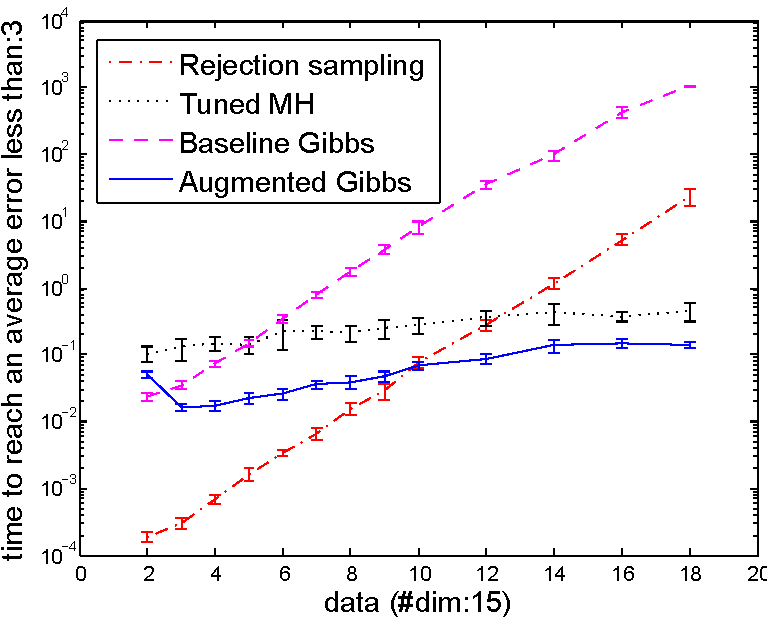
\includegraphics[scale=0.55]{plot/bppl_data_analysis_fit.pdf}
  \caption{}
  \label{fig:error-samples-bppl}
\end{subfigure}
\begin{subfigure}{.48\textwidth}
  \centering
  \hspace{5mm} 
  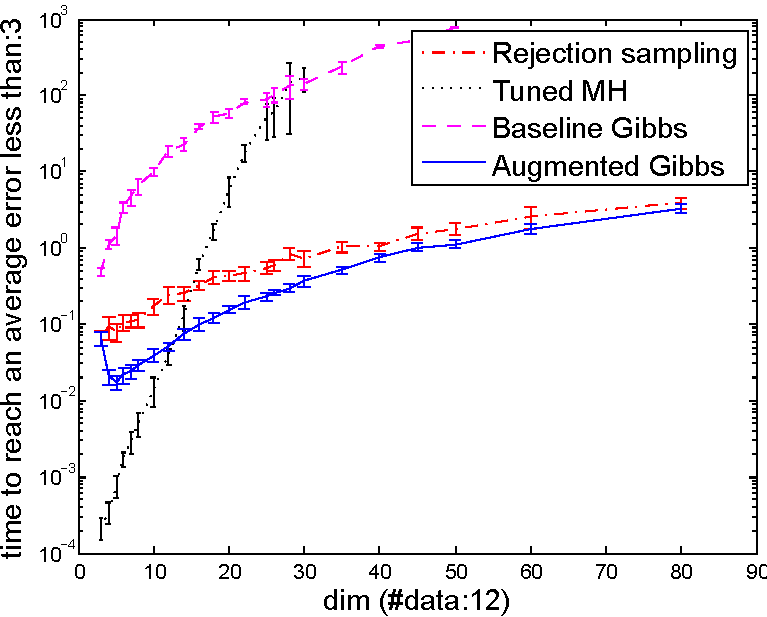
\includegraphics[scale=0.55]{plot/bppl_dim_analysis_fit.pdf}
  \caption{}
  \label{fig:error-samples-bppl}
\end{subfigure}
\centering
\begin{subfigure}{.48\textwidth}
  \centering
  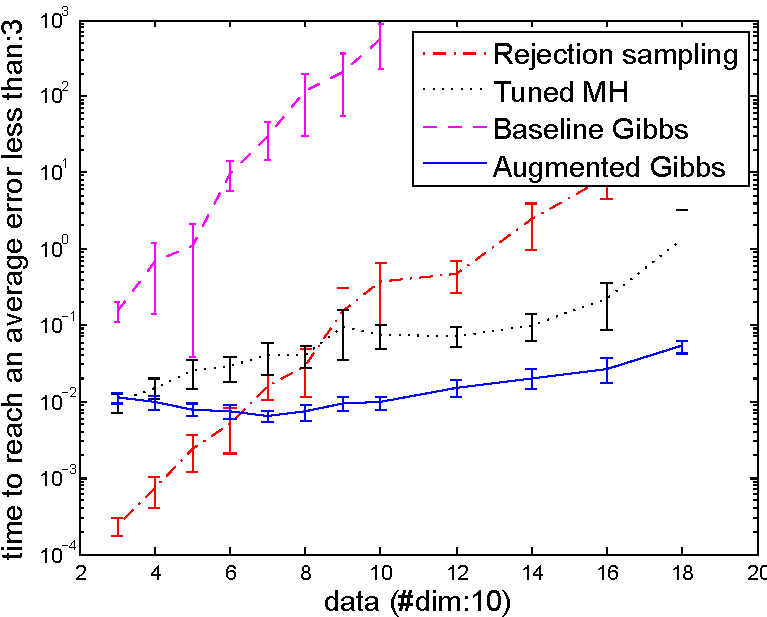
\includegraphics[scale=0.55]{plot/mmm_data_analysis2.pdf}
  \caption{}
  \label{fig:mmm_data_analysis}
\end{subfigure}
\begin{subfigure}{.48\textwidth}
  \centering
  \hspace{5mm} 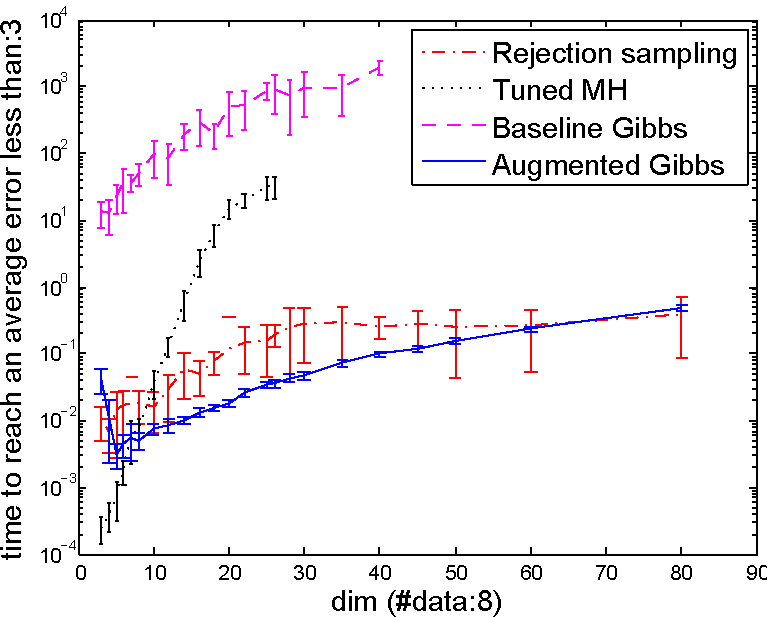
\includegraphics[scale=0.55]{plot/mmm_dim_analysis10.pdf}
  \caption{}
  \label{fig:mmm_dim_analysis}
\end{subfigure}
\vspace{-1mm}
\caption{\footnotesize Performance of Rejection/Metropolis-Hastings, baseline and augmented Gibbs on (a) \& (b) BPPL and (c) \& (d) MM models against different configurations of the number of observed data and the dimensionality of the parameter space.  Apart from low data size and/or dimensionality, in almost all cases, Augmented Gibbs takes orders of magnitude less time to achieve the same error as the other methods and this performance separation from competing algorithms increases in many cases with both the data size and dimensionality.}
\label{fig:results}
\vspace{-3mm}
\end{figure*}

For each combination of the parameter space dimensionality $D$ and the number 
of observed data $n$, we generate data points from each model and simulate the 
associated expected value of ground truth posterior distribution by running 
rejection sampling on a 4 core, 3.40GHz PC for 15 to 30 minutes.
Subsequently, using each algorithm, particles are generated and based on them, 
average absolute error between samples and the ground truth, $||\mathbb{E}[\boldsymbol\theta] - \boldsymbol\theta^*||_1$, is computed. 
The time till the absolute error reaches the threshold error 3.0 is recorded.
For each algorithm, three independent Markov chains are executed and the results are averaged.
The whole process is repeated 15 times and the results are averaged and standard errors are computed. 

We observe that
in both models, the behavior of each algorithm has a particular pattern 
(Figure~\ref{fig:results}). 
The speed of rejection sampling and consequently its mixing time deteriorates rapidly as the number of observations increases.%\footnote{For the same reason we were obliged to constrain the observations to less than 18 data points since beyond this, even after 30 minutes the number of samples taken to simulate the ground truth were not sufficient to allow a fair comparison between algorithms.}
The reason is that by observing new data, the posterior density tends to concentrate in smaller areas, 
leaving most of the space sparse and therefore hard to sample from by rejection sampling.

It is known that the efficiency of MH depends crucially on the tuning
of the \emph{proposal}.  We carefully tuned MH to reach the optimal
acceptance rate of 0.234~\cite{Roberts:97}.  The experimental results
show that MH is scalable in observations but its mixing time increases
rapidly as the dimensionality increases.  These results are rather
surprising since we expected that as an MCMC, MH does not suffer from
the curse of dimensionality as rejection sampling does.  A reason may
be that piecewise distributions can be non-smooth or broken (see
Figure~\ref{fig:mmm}) which is far from the characteristics of the
Gaussian \emph{proposal density} used in MH.

Efficiency of the baseline Gibbs sampling in particular decreases as data points increase since
this leads to an exponential blow-up in the number of partitions in the posterior density.
On the other hand, Augmented Gibbs is scalable in both data 
and dimension for both models. 
Interestingly, its efficiency even increases as dimensionality increases from 2 to 5 ---
the reason may be that proportional to the total number of posterior partitions, in lower dimensions the neighbors of each partition are not as numerous. 
For instance, regardless of the number of observed data in the 2 dimensional BPPL, each partition is neighbored by only two partitions (see Figure~\ref{fig:pref-up-down}) leading to a slow transfer between partitions. 
In higher dimensions however, this is not often the case.


%---------------------------%
%        conclusion           %
%---------------------------%
\section{Conclusion}
\label{sect:conclusion}
In this work, we showed how to transform piecewise likelihoods in
graphical models for Bayesian inference into equivalent mixture models
and then provide a blocked Gibbs sampling approach for this augmented
model that achieves an \emph{exponential-to-linear} reduction in space
and time compared to a conventional Gibbs sampler.  Unlike rejection
sampling and baseline Gibbs sampling, the time complexity of the
proposed Augmented Gibbs method does not grow exponentially with the
amount of observed data and yields faster mixing times in high
dimensions than Metropolis-Hastings.

Future extensions of this work can also examine application of this
work to non-Bayesian inference models (i.e., general piecewise
graphical models).  For example, some clustering models can be
formalized as piecewise models with latent cluster assignments for
each datum -- the method proposed here allows linear-time Gibbs
sampling in such models.  To this end, this work opens up a variety of
future possibilities for efficient asymptotically unbiased (Bayesian)
inference in expressive piecewise graphical models that to date have
proved intractable or inaccurate for existing (Markov Chain) Monte
Carlo inference approaches.


{\footnotesize
\section*{Acknowledgements}
NICTA is funded by the Australian Government as represented by
the Department of Broadband, Communications and the Digital
Economy and the Australian Research Council through the ICT
Centre of Excellence program.}

\clearpage

%\subsubsection*{References}
% \small{
\bibliographystyle{aaai} %{plain}%{plainnat}  
\bibliography{fastBayes} % \jobname}       % uses \jobname.bib, according to \jobname.tex
% }

\end{document}
